\subsection{OpenMP of the Jacobi Method}
The Jacobi method updates a new matrix from the values of an old one, and it is thus easily parallelizable. The program is paralellized using orphaning in openMP. The \texttt{\#pragma omp parallel} is inside the while loop described above. That has the obvious disadvantage that the worker team will be created and destroyed with each iteration, creating a lot of overhead that will reduce performance. To measure and analyze the performance and scaling behavior of the paralized implementations, we map the speed up as a function of the number of processors/therads used. To investigate the speed up, the program is sent through the Sun Studio Performance Analyzer tool in sequential mode to see the fraction of time f spent in the parallelized region, to facilitate a comparison with Amdahl's law. Amdahl's idealized law is used as a benchmark throughout the scaling analysis.

\begin{equation}
S(P)=\dfrac{T(1)}{T(P)}=\dfrac{1}{(f/P+1-f)}
\end{equation}

S(P) is the speed up. T(1) is the sequential execution time, P is the number of processors, T(P) is the execution time on P processors and f is the parallized fraction of the code. 
The speed up of the initial simple implementation is seen in figure \ref{fig:omp_scale1}. It is seen, that we experience some speed up on more processors, but it does stabilize quickly around 5 threads with a speed up factor of 1.15. The f value of 0.22 is rather low and clearly much of computation time is not spent in parallel, and when we compare it to Amdahl's law, it is clearly not performing well.

\begin{figure}[h!]
\centering
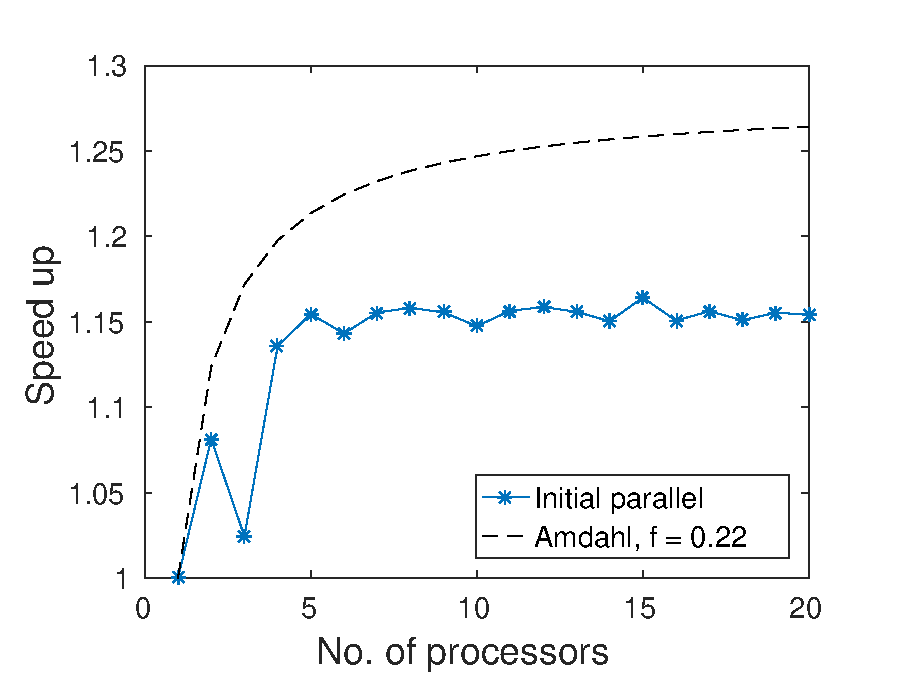
\includegraphics[width = 0.8\textwidth]{fig/speedup_omp.eps}
\caption{Scaling of the first parallelized version.}
\label{fig:omp_scale1}
\end{figure}

We now seek to improve the OpenMP parts of the code and to make the program better suited for running in parallel. First we realize, that right now we are only running the Jacobi calculation in parallel, and it can be seen that the program spent a lot of time on calculating the Frobenius square and updating the old matrix. Furthermore, initializing the parallel region in each iteration of the is not optimal, so we seek to make the whole loop parallel. This can all be viewed in the code in the omp2 function. The specific changes are described in the following: The parallel initialization is moved outside the loop with the shared variables u,uo,f,N,delta2, checksum, k, d and kmax. The Jacobi calculation is parallel using pragma omp for as in the simple version, the checksum is also parallel by using a omp for loop with reduction on checksum, so we do not experience any simultaneous update errors. The loop iteration variable k loop variable and checksum normalization is inside a pragma omp master directive. In the end we set a barrier to make sure, that the whole loop is finished and the loop variables checksum and k updated.


					
					

We now end up with a much higher parallel fraction f of 0.93. In figure \ref{fig:omp2_scale} the scaling behavior is seen for the more optimized version. The speed up is clearly much bigger stablizing at 7 threads with a bit less than a factor 4. It does however not keep up with Amdahl's law.

\begin{figure}[h!]
\centering
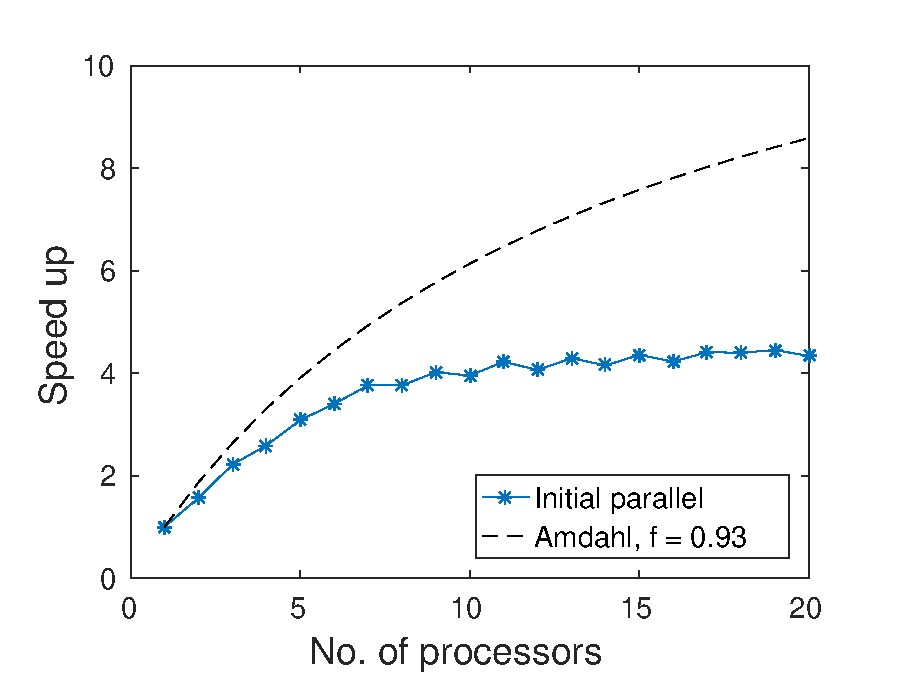
\includegraphics[width = 0.8\textwidth]{fig/speedup_omp2.eps}
\caption{Scaling of the second parallelized version of the whole computational while loop.}
\label{fig:omp2_scale}
\end{figure}

As a final step, we seek to optimize the program even more by implementing a parallization of the memory allocation of the matrices. This can be seen in figure \ref{fig:omp3_scale}. Now the f actually becomesas high as 0.955. This also impact the speed up scaling and the parallel program is just more effective in general with the parallel memory allocation and it keeps up with Amdahl's law for the first 18 processors. It looks like it begins to stabilize around 18 threads, but it is hard to conclude that, since the speed up is just slightly below the benchmark.

\begin{huge}
DESCRIBE HOW
\end{huge}

\begin{figure}[h!]
\centering
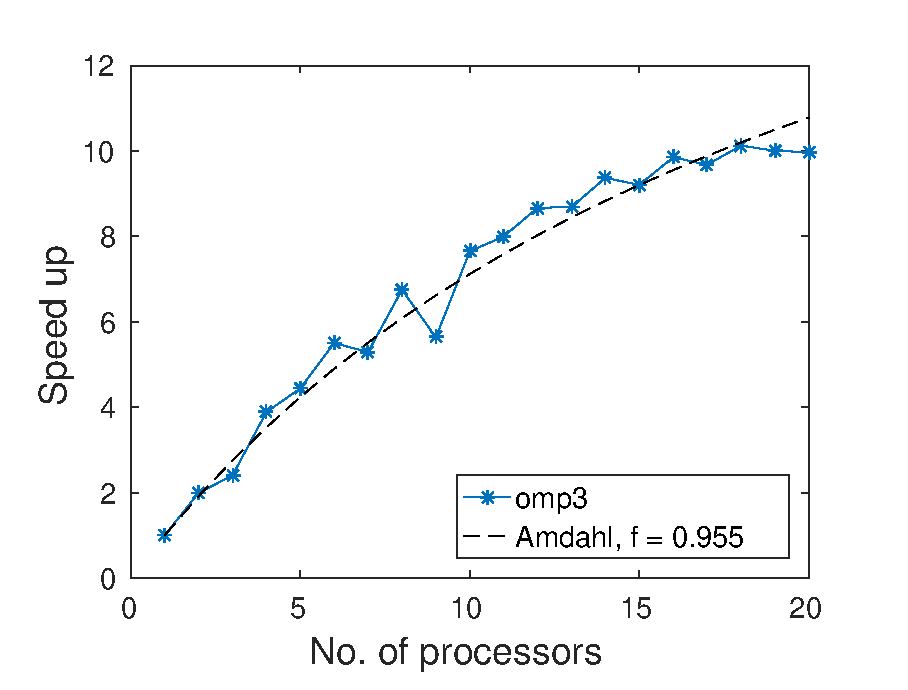
\includegraphics[width = 0.8\textwidth]{fig/speedup_omp3.eps}
\caption{Speed-up scaling of the third parallelized version, which includes parallel memory allocation.}
\label{fig:omp3_scale}
\end{figure}


In the end, we would like to compare the efficiency of the three different degrees of parallel implementation. This is done by computing the efficiency, which is the speed up increase per added thread. Figure \ref{fig:omp_eff} clearly shows how different the efficiency are for the three different implementations. The simple implemenation clearly falls of right at the beginning, where the efficiency drops to a little higher than 50\% already at thread nr. 2, which is obvious since the speed up factor is only slightly above 1. For the case of the more optimized implementation, it is clear that the omp3 version reigns supreme, and it does not reach 50\% effiency before the 19th to 20th added thread, which makes sense, since we saw in the speed-up scaling that it started to stagnate at that point. Meanwhile the omp2 parallelization already reaches 50\% around 7-8 threads.

\begin{figure}[h!]
\centering
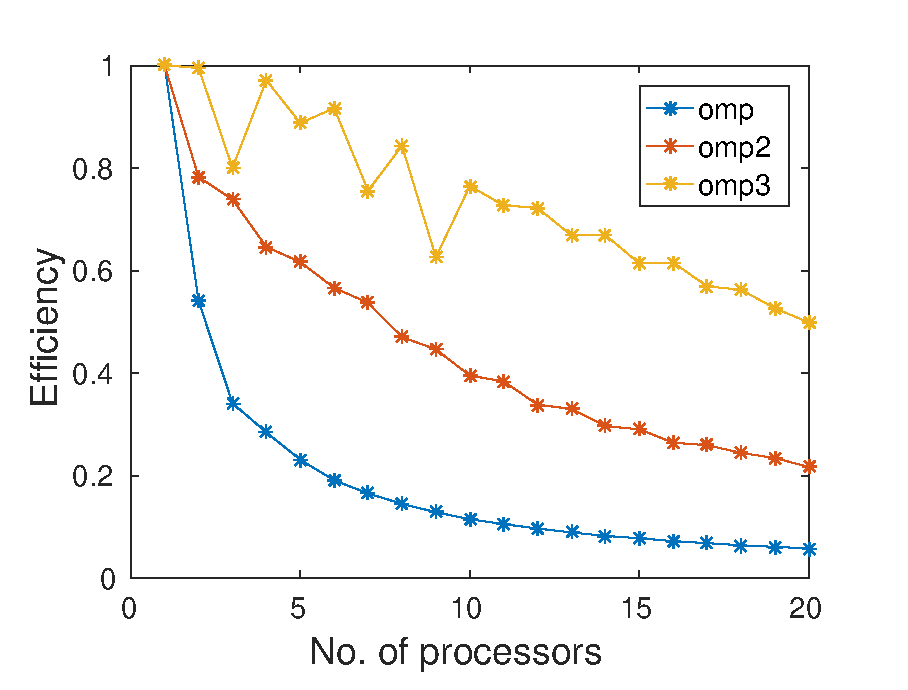
\includegraphics[width = 0.8\textwidth]{fig/efficiency_omp_omp2_omp3.eps}
\caption{Effiency plot of the three parallel versions.}
\label{fig:omp_eff}
\end{figure}
